%% BioMed_Central_Tex_Template_v1.06
%%                                      %
%  bmc_article.tex            ver: 1.06 %
%                                       %

%%IMPORTANT: do not delete the first line of this template
%%It must be present to enable the BMC Submission system to
%%recognise this template!!

%%%%%%%%%%%%%%%%%%%%%%%%%%%%%%%%%%%%%%%%%
%%                                     %%
%%  LaTeX template for BioMed Central  %%
%%     journal article submissions     %%
%%                                     %%
%%          <8 June 2012>              %%
%%                                     %%
%%                                     %%
%%%%%%%%%%%%%%%%%%%%%%%%%%%%%%%%%%%%%%%%%
%\usepackage{lineno}
%\linenumbers
%
%\doublespacing

%%%%%%%%%%%%%%%%%%%%%%%%%%%%%%%%%%%%%%%%%%%%%%%%%%%%%%%%%%%%%%%%%%%%%
%%                                                                 %%
%% For instructions on how to fill out this Tex template           %%
%% document please refer to Readme.html and the instructions for   %%
%% authors page on the biomed central website                      %%
%% http://www.biomedcentral.com/info/authors/                      %%
%%                                                                 %%
%% Please do not use \input{...} to include other tex files.       %%
%% Submit your LaTeX manuscript as one .tex document.              %%
%%                                                                 %%
%% All additional figures and files should be attached             %%
%% separately and not embedded in the \TeX\ document itself.       %%
%%                                                                 %%
%% BioMed Central currently use the MikTex distribution of         %%
%% TeX for Windows) of TeX and LaTeX.  This is available from      %%
%% http://www.miktex.org                                           %%
%%                                                                 %%
%%%%%%%%%%%%%%%%%%%%%%%%%%%%%%%%%%%%%%%%%%%%%%%%%%%%%%%%%%%%%%%%%%%%%

%%% additional documentclass options:
%  [doublespacing]
%  [linenumbers]   - put the line numbers on margins

%%% loading packages, author definitions

%\documentclass[twocolumn]{bmcart}% uncomment this for twocolumn layout and comment line below
\documentclass[]{bmcart}
%%% Load packages
\usepackage{amsthm,amsmath}
\usepackage{graphicx}
\usepackage{hyperref}
\hypersetup{colorlinks=false}
\usepackage{natbib}
\usepackage{booktabs}
\usepackage{amsfonts}
\usepackage{bm}
\usepackage{tikz, tkz-euclide}
\usetikzlibrary{matrix,arrows,decorations.pathmorphing, arrows,chains,matrix,positioning,scopes, decorations.markings, patterns,bayesnet, calc}
\newcommand{\vt}{\bm{t}}
\newcommand{\vs}{\bm{s}}
\newcommand{\va}{{\alpha}}
\newcommand{\vb}{\bm{\beta}}
%\newcommand{\vd}{\bm{\delta}}
\newcommand{\vd}{{D}}
\newcommand{\vm}{{\mu}}
\newcommand{\vw}{\bm{w}}
\newcommand{\vx}{\bm{x}}
\newcommand{\lo}[1]{{\log}\left(#1\right)}
\newcommand{\ex}[1]{{\exp}\left(#1\right)}
\usepackage[linesnumbered,ruled]{algorithm2e}
\newcommand{\vD}{\bm{D}}
%\RequirePackage[authoryear]{natbib}% uncomment this for author-year bibliography
%\RequirePackage{hyperref}
\usepackage[utf8]{inputenc} %unicode support
%\usepackage[applemac]{inputenc} %applemac support if unicode package fails
%\usepackage[latin1]{inputenc} %UNIX support if unicode package fails


%%%%%%%%%%%%%%%%%%%%%%%%%%%%%%%%%%%%%%%%%%%%%%%%%
%%                                             %%
%%  If you wish to display your graphics for   %%
%%  your own use using includegraphic or       %%
%%  includegraphics, then comment out the      %%
%%  following two lines of code.               %%
%%  NB: These line *must* be included when     %%
%%  submitting to BMC.                         %%
%%  All figure files must be submitted as      %%
%%  separate graphics through the BMC          %%
%%  submission process, not included in the    %%
%%  submitted article.                         %%
%%                                             %%
%%%%%%%%%%%%%%%%%%%%%%%%%%%%%%%%%%%%%%%%%%%%%%%%%


%\def\includegraphic{}
%\def\includegraphics{}



%%% Put your definitions there:
\startlocaldefs
\endlocaldefs

%%% Begin ...
\begin{document}

%%% Start of article front matter
\begin{frontmatter}

\begin{fmbox}
\dochead{Research}

%%%%%%%%%%%%%%%%%%%%%%%%%%%%%%%%%%%%%%%%%%%%%%
%%                                          %%
%% Enter the title of your article here     %%
%%                                          %%
%%%%%%%%%%%%%%%%%%%%%%%%%%%%%%%%%%%%%%%%%%%%%%

\title{Predicting the spread and persistence of genetically modified dominant sterile male mosquitoes}

%%%%%%%%%%%%%%%%%%%%%%%%%%%%%%%%%%%%%%%%%%%%%%
%%                                          %%
%% Enter the authors here                   %%
%%                                          %%
%% Specify information, if available,       %%
%% in the form:                             %%
%%   <key>={<id1>,<id2>}                    %%
%%   <key>=                                 %%
%% Comment or delete the keys which are     %%
%% not used. Repeat \author command as much %%
%% as required.                             %%
%%                                          %%
%%%%%%%%%%%%%%%%%%%%%%%%%%%%%%%%%%%%%%%%%%%%%%

\author[
   addressref={aff1},                   % id's of addresses, e.g. {aff1,aff2}
   corref={aff1},                       % id of corresponding address, if any
%   noteref={n1},                        % id's of article notes, if any
   email={adrien.ickowicz@csiro.au}   % email address
]{\inits{A}\fnm{Adrien} \snm{Ickowicz}}
\author[
   addressref={aff1},
   email={scott.foster@csiro.au}
]{\inits{SD}\fnm{Scott D} \snm{Foster}}
\author[
   addressref={aff1},
   email={geoff.hosack@csiro.au}
]{\inits{GR}\fnm{Geoffrey R} \snm{Hosack}}
\author[
   addressref={aff1},
   email={keith.hayes@csiro.au}
]{\inits{KR}\fnm{Keith R} \snm{Hayes}}
%%%%%%%%%%%%%%%%%%%%%%%%%%%%%%%%%%%%%%%%%%%%%%
%%                                          %%
%% Enter the authors' addresses here        %%
%%                                          %%
%% Repeat \address commands as much as      %%
%% required.                                %%
%%                                          %%
%%%%%%%%%%%%%%%%%%%%%%%%%%%%%%%%%%%%%%%%%%%%%%

\address[id=aff1]{%                           % unique id
  \orgname{CSIRO Data 61}, % university, etc                   %
  %\postcode{}                                % post or zip code
  \city{Hobart},                              % city
  \cny{Australia}                                    % country
}

%%%%%%%%%%%%%%%%%%%%%%%%%%%%%%%%%%%%%%%%%%%%%%
%%                                          %%
%% Enter short notes here                   %%
%%                                          %%
%% Short notes will be after addresses      %%
%% on first page.                           %%
%%                                          %%
%%%%%%%%%%%%%%%%%%%%%%%%%%%%%%%%%%%%%%%%%%%%%%

\begin{artnotes}
%\note{Sample of title note}     % note to the article
%\note[id=n1]{Equal contributor} % note, connected to author
\end{artnotes}

\end{fmbox}% comment this for two column layout

%%%%%%%%%%%%%%%%%%%%%%%%%%%%%%%%%%%%%%%%%%%%%%
%%                                          %%
%% The Abstract begins here                 %%
%%                                          %%
%% Please refer to the Instructions for     %%
%% authors on http://www.biomedcentral.com  %%
%% and include the section headings         %%
%% accordingly for your article type.       %%
%%                                          %%
%%%%%%%%%%%%%%%%%%%%%%%%%%%%%%%%%%%%%%%%%%%%%%

\begin{abstractbox}

\begin{abstract} % abstract
\parttitle{Background} Reproductive containment provides an opportunity to implement a staged-release strategy for genetic control of malaria vectors, in particular allowing predictions about the spread and persistence of (self-limiting) sterile and male-biased strains to be compared to outcomes before moving to (self-sustaining) gene-drive strains.
\parttitle{Methods} We: (i) describe a diffusion-advection-reaction model of the spread and persistence of a single cohort of male mosquitoes; (ii) elicit informative prior distributions for model parameters, for wild type (WT) and genetically modified dominant sterile strains(DSM); (iii) estimate posterior distributions for wild type strains using data from published Mark Recapture Release (MRR) experiments, with inference performed through a delayed rejection adaptive Metropolis algorithm; and, (iv) weight prior distributions in order to make predictions about genetically modified strains using Bayes factors calculated for the wild type strains.
\parttitle{Results} If a single cohort of 5000 genetically modified dominant sterile male mosquitoes are released at the same location as the previous MRR experiments with WT, there is a 90\% probability that the expected number of released mosquitoes will fall below 1 in 10 days, and that by 12 days there will be a 99\% probability that no mosquitoes will be found more than 150 meters from the release location.
\parttitle{Conclusions} Spread and persistence models should form a key component of risk assessments of novel genetic control strategies for malaria vectors. Our predictions, used in an independent risk assessment, suggest genetically modified sterile male mosquitoes will remain within the locality of the release site, and persist for a very limited amount of time. Data gathered following the release of these mosquitoes will enable us to test the accuracy of these predictions and also provide a means to update parameter distributions for genetic strains in a coherent (Bayesian) framework. We anticipate this will provide additional insights about how to conduct probabilistic risk assessments for the stage-released of genetically modified mosquitoes.
\end{abstract}

%%%%%%%%%%%%%%%%%%%%%%%%%%%%%%%%%%%%%%%%%%%%%%
%%                                          %%
%% The keywords begin here                  %%
%%                                          %%
%% Put each keyword in separate \kwd{}.     %%
%%                                          %%
%%%%%%%%%%%%%%%%%%%%%%%%%%%%%%%%%%%%%%%%%%%%%%

\begin{keyword}
\kwd{entomological survey data}
\kwd{sterile male}
\kwd{expert elicitation}
\kwd{Bayesian hierarchical model}
\kwd{monitoring}
\end{keyword}

% MSC classifications codes, if any
%\begin{keyword}[class=AMS]
%\kwd[Primary ]{}
%\kwd{}
%\kwd[; secondary ]{}
%\end{keyword}

\end{abstractbox}
%
%\end{fmbox}% uncomment this for twcolumn layout

\end{frontmatter}

%%%%%%%%%%%%%%%%%%%%%%%%%%%%%%%%%%%%%%%%%%%%%%
%%                                          %%
%% The Main Body begins here                %%
%%                                          %%
%% Please refer to the instructions for     %%
%% authors on:                              %%
%% http://www.biomedcentral.com/info/authors%%
%% and include the section headings         %%
%% accordingly for your article type.       %%
%%                                          %%
%% See the Results and Discussion section   %%
%% for details on how to create sub-sections%%
%%                                          %%
%% use \cite{...} to cite references        %%
%%  \cite{koon} and                         %%
%%  \cite{oreg,khar,zvai,xjon,schn,pond}    %%
%%  \nocite{smith,marg,hunn,advi,koha,mouse}%%
%%                                          %%
%%%%%%%%%%%%%%%%%%%%%%%%%%%%%%%%%%%%%%%%%%%%%%

%%%%%%%%%%%%%%%%%%%%%%%%% start of article main body
% <put your article body there>

%%%%%%%%%%%%%%%%
%% Background %%
%%
\section{Background}
%\paragraph{Context}
Over the last thirty years conventional control strategies have reduced the global incidence rate of malaria. The efficacy of these strategies, however, appears to be waning. Global malaria incidence rates have barely changed since 2014, stalling around 57 cases per 1000 population at risk despite increased expenditure on elimination and prevention between from 2014 to 2017 \citep{WHO2019}. Consequently, the World Health Organisation predicts that morbidity targets for 2020, 2025 and 2030 will not to be met without significant improvements in vector control and chemoprevention.

Laboratory studies and modelling indicate that novel control strategies that use gene drives to force effector genes through vector populations to suppress them, or render them unable to transmit plasmodium parasites, could augment conventional strategies and significantly improve current rates of malaria control \citep{Gabrieli2014,Beaghton2017, CarballarLejarazu2020,Simoni2020}. As with many novel technologies, however, the safety of genetic control methods is uncertain, and the potential for spread and ecosystem-wide impacts makes gene-drives contentious \citep{Ledord2015,Champer2016}.

To date, all research on gene-drive modified mosquitoes (GDMMs) has been conducted in laboratories under strict physical, ecological, reproductive and/or molecular containment \citep{Akbari2015}. Current guidance recommends that if containment is to be relaxed it should be done in a ``phased-release'' strategy wherein data is gathered, risks are evaluated, and containment is gradually lifted in a step-wise fashion if and when the risks are deemed acceptable \citep{WHOTDRFNIH2014,NASEM2016}. The possibility of long-distance dispersal \citep{Huestis2019} and biosecurity concerns with large semi-field enclosure, however, may erode confidence in strategies that try to gradually lift ecological or physical containment. 

Genetic and reproductive containment strategies on the other hand may be more amenable to a gradual-release strategy, and several approaches are currently being pursued \citep{Klein2012,Galizi2014,Nash2019}. In this paper we focus on the spatio-temporal dynamics that govern the spread and persistence of a single cohort of genetically modified, Dominant Sterile Male (DSM) \textit{Anopheles coluzzii} mosquitoes released in a small village in Burkina Faso. These mosquitoes are reproductively contained, and represent the first stage in a three-stage pathway to malaria vector control using a gene drive that results in a male-biased sex ratio \citep{Beaghton2017a,North2019}.

%Pest insects represent a major threat to public health, to food security as well as to the economics. Constant effort is being made to develop or improve control strategies for the management of pest insects. Such management aims to maintain insects at low levels that do not represent risks for health or economics, while satisfying environmentally respectful toxicological and ecological requirements. Planning of efficient control strategies requires in-depth knowledge of the insect’s biology and ecology \cite{Way2000}. In particular, it is essential to have accurate estimates of parameters of biological and ecological relevance like population size and distribution, dispersal capacity, as well as good understanding of the underlying processes governing the dynamics of the population in time and space.

%\paragraph{Mass release of organism can be an effective tool for pest insects management}
%Sterile insect techniques (SIT) can be traced back to the work of Knipling \cite{Knipling1959} as they discovered that the abundance of mosquitoes could be reduced if females mate with sterile males. In this context, sterile insect techniques are a promising control method for pest-insect populations. SIT consists in releasing a large number of reared sterilized males to compete with wild males for female insemination. Females inseminated by sterile males produce no offspring or non-viable ones, leading to the reduction of the mosquito population in one or two generations. Genetic control is the next natural step, as while very similar to SIT control, the use of a lethal or disease-refractory gene can lead to either abundance reduction or a majority of disease-refractory insects in the population \cite{Dufourd2016}. These genetic control management approaches have been successfully (or showing promising early results) used in various cases \cite{Catteruccia2000, Bellini2007, Gabrieli2014}. 

%\paragraph{We need to predict the outcomes prior to the release in order to assess efficacy and safety}
%A major advantage of genetic control, is its species-specific nature. With such methods, the target-species is controlled without affecting other species or the surrounding environment. Further, the involvement of living organisms allow to reach areas that other cannot be controlled using other methods due to physical barriers or lack on the ecological knowledge of the species. Moreover, there are no health concerns for humans due to chemical residues meeting the requirements of insecticide based management. Despite these benefits biological control can be difficult to implement. Indeed, the natural candidates are usually expensive and sometimes difficult to rear in large abundance. In addition, evaluating the establishment of the candidate insect in a new environment is difficult (Is there a risk of invasion? Can it survive in the new environment?). Further, a good understanding on the insect biology and its interactions with the environment is essential for its success. In particular, for efficient control strategy, one should address the following questions: (i) When and where should the modified insects be released? (ii) How many sterile insects should be introduced to ensure efficient control? (iii) At what frequency should the releases occur? Planning efficient biological control is not straightforward. To optimize such strategies, mathematical models can provide a useful tool to study the system and simulate various scenarios.

%\paragraph{Modeling of spread and persistence of mosquitoes can be done via different approaches}
%The modeling of the spread and persistence of a population of  mosquitoes is usually performed using either an empirical model based on experimental data with particular experimental conditions, or a theoretical model, where a mathematical structure is used to model the general dynamics. The empirical models are accurate, in that they describe the population accurately, but are very specific to the population measured. The mathematical models can be generalized to many populations but the trade-off is the accuracy.  

%\paragraph{We use data from mark recapture release and elicitation to run an inference for WT mosquitoes model parameters}
In our analysis the spatio-temporal dynamics of DSM mosquitoes are driven by: (i) a diffusion process that accounts for the dispersal capacity of the insects; (ii) an advection process that accounts for the attraction of individuals to swarms, and (iii) a reaction process that accounts for the death of sterile male mosquitoes. These processes can be described mathematically by a partial differential equation (PDE) of the advection-diffusion-reaction type, which models how the distribution of mosquitoes in time and space is affected by a chemo-attractant present in the environment. Models of this type have also been widely used within the environmental and ecological literature. In particular, such models have been used before to model mosquitoes, for example the dispersal of \emph{Aedes albopictus} in Reunion Island using a similar type of parabolic PDE \citep{Dufourd2012}.

Our objective is to predict the spread and persistence of the genetically modified mosquitoes ahead of a proposed field release. These predictions are an important component of an independent risk assessment conducted prior to the field release \cite{Hayes2015a} that assessed the risk of vecotr-borne disease transmission \cite{Hosack2020}, and could also help to inform the design of a post-release monitoring strategy. Our approach implements the Bayesian paradigm; we elicit the prior distribution of model parameters from relevant experts, for both the wild type mosquito (WT) and its DSM counterpart. We obtain the posterior model parameter values for the WT parameters using the results of mark-release-recapture (MRR) experiments conducted by \cite{Epopa2017}. We then use Bayesian model averaging to predict the spread and persistence of DSM mosquitoes. 

\section{Methods}

\subsection{PDE model}

%\paragraph{Description of the model type/form}
The literature review conducted by \cite{Cummins2012} suggests that the behaviour of host-seeking mosquitoes can be categorised as: (i) \emph{plume finding} in which flight direction is either random (kinesis), determined by visual features in the absence of wind or deliberately upwind, downwind or crosswind (anemotaxis) when wind is present; and, (ii) \emph{plume tracking}, where once the mosquito detects an odour plume, flight direction is deliberately upwind, or possibly determined by the odour gradient in windless conditions, in order to find the odour source (positive chemotaxis). More details on the properties of these search strategies can be found in \cite{Pasternak2009}. 

In this analysis, we assume that village compounds (groups of closely spaced houses) provide a source of CO$_2$ that acts as an attractant for female \emph{Anopheles gambiae sensu strictu} and \emph{Anopheles coluzzi} mosquitoes \cite{DeJong1995, Majeed2017}. We further assume that male mosquitoes swarm in places where the probability of encountering receptive females is highest \citep{Diabate2015}, hence swarms occur in and around compounds (as evident in Figure 1 of \citep[][]{Epopa2017}). Consequently, high concentrations of attractant result in flights that (on average) are closer to the direction of the nearest compound for both males and females. Conversely, low concentrations have less influence on the mosquitoes and result in greater variability in flight direction. We do not incorporate the effect of wind speed or direction into the analysis (we assume the local dispersal dynamics are not greatly affected by the wind at this spatial scale), and also assume that the attraction process is not influenced by the number of mosquitoes.

With these assumptions we developed an advection-diffusion-reaction model to describe the expected number of male WT and DSM mosquitoes,
\begin{align}
\lambda_{\vt} &= \vd \Bigl[ \lambda_{\vs \vs}-\va \cdot \nabla_{\vs} \left( \lambda U(\vs)\right) \Bigr]-\vm \lambda, \label{mod3}
\end{align}
with the following boundary conditions (Neumann reflecting conditions):
\begin{align}
\frac{\partial \lambda}{\partial s} &= 0
\end{align}
where $U(\vs)$ is a function that describes the strength of mosquito attraction at location $s$, and $\va$ enables us to modulate the effect of the utility function on the overall attraction. Utility functions like this have been used in similar ecological contexts to describe an attractive or repulsive flux \citep{Moorcroft2008}.

In this model we use swarm sites as centers of attraction and assume that the strength of attraction decays according to a squared-sum exponential decay kernel
\begin{eqnarray}
U(\vs) &=& \sum_{\vs_\ell \in \mathcal{L}} \exp\Big[  - \frac{|\vs - \vs_\ell |^2}{\sigma^2}\Big]
\end{eqnarray}
where $\mathcal{L}$ are the known swarm locations (identified prior to the MRR experiment \citep{Epopa2017}) and $\sigma$ is an unknown parameter that controls the range of attraction - that is the distance beyond which the attraction of a swarm site $\vs_\ell$ for a mosquito is negligible. 

The theoretical solution to the partial differential equation~\ref{mod3} is the expected number of male mosquitoes at time $t$ and location $\vs=(\mathrm{easting},\mathrm{northing})$. The partial derivatives are denoted $\lambda_{\vt}$ (with respect to time) and $\lambda_{\vs \vs}$ (with respect to location). Because we use a numerical solver, we define a grid over the spatial domain. Each grid cell is therefore one areal unit. In this study, an areal unit is a square of 100 m$^2$ of area. All process model parameters are summarised in Table \ref{tble:parameters}.

\begin{table}[ht]
\centering
\begingroup

\begin{tabular}{cp{60mm}c}
\hline
Name & Description & Units \\
\hline
$\va$ & Attractiveness of swarms & reward$^-1$.$m^-1$\\
%$\vb$ & Decay of attractiveness & \colorbox{orange!30}{??} \\
$\vm$ & Male mosquito mortality rate &  day$^{-1}$\\ 
$\lambda$ & The expected number of male mosquitoes & Number of mosquitoes per areal unit \\ 
$\vd$ & Isotropic diffusion coefficient & $m^2$.day$^-1$\\ 
$\sigma$ & Decay of attraction to swarm sites  & $m$\\
\hline
\end{tabular}
\endgroup
\caption{\label{tble:parameters} The parameters and units of the diffusion-advection-reaction model for sterile male mosquitoes.} 
\end{table}

\subsection{Data}
%\paragraph{MRR data - what parameters is the data talking to}
In this analysis we use the results of five MRR experiments \cite{Epopa2017} wherein approximately 5000 adult male WT mosquitoes, marked with a colored powder, were released two hours before swarming (around 4pm), at three different locations, on five different dates (Table~\ref{tab:relLoc}). Mosquitoes were recaptured in three ways via: (i) swarm sampling in the evening (times were not specified, but we assume the sampling occurred between 7pm and 9pm); (ii) Pyrethroid Spray Catches in the morning inside houses; and, (iii) placement of humidified clay pots within rooms within houses, that were subsequently checked in the morning (between 6am-7am). All releases and re-captures sites were geo-located allowing for a spatial model to be used.

Recaptures were performed for seven days after release for all experiments except the first where recaptures were performed for five days. We used the results of the first four MRR experiments to derive posterior estimates of male WT model parameters, reserving the results of the fifth experiment to compare with model predictions.

% latex table generated in R 3.4.1 by xtable 1.8-2 package
% Fri Oct 13 08:25:21 2017
\begin{table}[ht]
\centering
\begingroup\small
\begin{tabular}{|cccccccc|}
\hline
MRR & Date & Release site & Longitude & Latitude & N released & N captured & Distance\\ 
\hline
1 & 2013-10-09 & A & -4.4724 & 11.2347 & 1146 & 32 & 140\\ 
1 & - & B & -4.4755 & 11.2342 & 1158 & 9 & 344\\ 
1 & - & C & -4.4718 & 11.2318 & 1103 & 6 & 205\\ 
2 & 2014-05-07 & A & -4.4724 & 11.2347 & 1878 & 6 & 94\\ 
2 & - & B & -4.4755 & 11.2342 & 1655 & 1 & 266\\ 
2 & - & C & -4.4718 & 11.2318 & 1734 & 1 & 193\\ 
3 & 2014-09-04 & A & -4.4724 & 11.2347 & 1665 & 56 & 133\\ 
3 & - & B & -4.4755 & 11.2342 & 1673 & 4 & 440\\ 
3 & - & C & -4.4718 & 11.2318 & 1684 & 13 & 205\\ 
4 & 2015-04-09 & A & -4.4724 & 11.2347 & 2107 & 1 & 55\\ 
4 & - & B & -4.4755 & 11.2342 & 2013 & 3 & 386\\ 
4 & - & C & -4.4718 & 11.2318 & 1953 & 18 & 190\\ 
5 & 2015-10-09 & C & -4.4724 & 11.2347 & 5992 & 18 & 141\\ 
\hline
\end{tabular}
\endgroup
\caption{Summary of the MRR experiments conducted by \cite{Epopa2017} in Burkina Faso. The last column presents the average distance for recapture (in meters). We use the results of the first four experiments to parameterise our model and calculate Bayes factor for expert-derived priors, and use the fifth MRR experiment is to validate the model predictions.} 
\label{tab:relLoc}
\end{table}

\subsection{Priors}
\subsubsection{Process model}
%\paragraph{Prior of parameters: elicitation data}
A key challenge when conducting risk assessments of a novel technology is the lack of empirical information. Without any operational history from which success and failure rates might be estimated, quantitative risk predictions must (at least initially), be based on the testable predictions of domain experts. The Bayesian inference paradigm encourages the careful elicitation of prior information, and provides a coherent mechanism for updating this information as data becomes available \citep{Lindley2000}. The experimental observations and expert elicitation, however, must be independent but carefully aligned for this process to work.

For this analysis we carefully elicited opinions on the mortality rate and dispersal distance of WT and DSM male mosquitoes from four independent experts who were not involved in the development of the DSM mosquitoes \cite{Hayes2015a}. Prior to the elicitation, experts were provided information on the genetic construct (originally incorporated into the G3 laboratory colony strain of \textit{An. gambiae}) and were told that the genetically modified strain would be repeatedly backcrossed with wild type mosquitoes captured in the vicinity of a biosecure laboratory in order to gradually replace the G3 genetic background with that of the locally originated strain. The location of the laboratory was provided to each expert but the species of local WT mosquitoes was not specified. For the mortality rate, experts were proposed to answer questions about either the probability of mortality, the probability of survival, or the life expectancy. All responses were converted to an estimate of the daily probability of survival ($p$) which was then converted to the mortality rate parameter ($\mu = -\log(p)$) used in the PDE model.

The model's diffusion parameter ($\vd$) was not elicited directly but calculated using the experts' prior opinion on the average daily dispersal distance ($d$) of male mosquitoes. All experts agreed that a log-normal distribution provided the most appropriate description of their uncertainty for both WT and DSM strains. The model's prior diffusion parameter was subsequently calculated using the relation $\vd = d^2/\pi t$ (see Appendix for a detailed derivation). The geographical and temporal context of the elicitation was carefully prescribed, including a standardized time frame (dispersal over a one day period), so that all experts' opinions could be combined.

The model's two chemotaxis-related parameters are: (i) the relative strength of attraction towards the source of the attractant that a mosquito experiences at a location ($\va$), with units $m^{-1} R^{-1}$ where $m$ is the distance in meters between the location and the source and $R$ is a measure of the ``reward'' at the source, often expressed as the concentration of $CO_2$ for female mosquitoes; and, (ii) the distance beyond which a mosquito is negligibly attracted to a swarm site, called the range ($\sigma$) with units $m$. The attractiveness of a swarm site at distance $\sigma$ from a mosquito is roughly 38\% of its attractiveness at zero distance.

Finding prior information on these parameters proved difficult for the particular setting of this model, in particular for $\va$. We therefore chose a very broad prior distribution for $\va$ that spans several orders of magnitude, from $1\%$ (1st percentile) to $140\%$ (99th percentile) of the attraction at the source. For the range $\sigma$ defined the same way we do, different articles on related species provide values ranging from $3$m \cite{McIver1989}, to $18$m for single baiting or over $36$m for double baiting \cite{Gillies1972}, or even $40$m \cite{Zhu2015}. We therefore used a log-normal distribution for this prior with positive probability across all these possibilities (Table~\ref{tble:prior}). 

\subsubsection{Observation model}
An important advantage of the Bayesian paradigm is that it allows us to develop more realistic hierarchical models that capture uncertainty in the biological and physical processes that drive a phenomenon, as well as the uncertainty associated with the measurement process with which these processes are observed. In this context, this allows us to reflect the uncertainty about how many mosquitoes any particular trap will catch given a known number of mosquitoes in the proximity of the trap.

Here we represent the observation model uncertainty using three, trap-specific, catchability parameters, denoted $p_{cfr}$ for clay-pots, $p_{psc}$ for insecticide spraying and $p_{ss}$ for swarm sampling. These parameters define the probability of catching a mosquito given that it was in close proximity of the trap at the time of sampling \cite{Martin2005a}. Note that prior and posterior estimates of these parameters depend on the model resolution because the definition of ``close proximity'' is determined by the resolution of the raster (i.e. the grid cell size) over which the PDE model is numerically solved. Hence all predictions must be made at the same resolution used for solving the PDE and updating the prior distributions. 

The priors for the catchability parameters were chosen according to the following principles:
\begin{itemize}
\item For $p_{ss}$, a beta distribution with parameters $\alpha_{ss} = 10$ and $\beta_{ss} = 20$ (meaning on average one third of the mosquitoes in the swarm are caught, following the standard operating procedures of the MRR experiment, which requires one third of the swarm to be captured).
\item For $p_{psc}$, a beta distribution with parameters $\alpha_{psc} = 1.4$ and $\beta_{psc} = 1$. This prior was chosen because the PSC procedure involves spraying an entire room and capturing all the dead mosquitoes in the room. The PDE model, however, is specified at a resolution of the compounds which on average have $1.4$ rooms. We assume that each room has on average the same number of male mosquitoes.
\item For $p_{cfr}$, assuming this is the least efficient method but not having more information we deliberately selected a fairly low informative prior. So we chose a beta distribution with parameters $\alpha_{cfr} = 1$ and $\beta_{cfr} = 1$.
\end{itemize} 
A complete list of process and observation model priors and their sources is summarised in Table \ref{tble:prior}.

\begin{table}[h]
\centering
\begingroup\small
\begin{tabular}{|c|ccc|}
\hline
Parameter & Prior parameters & Prior distribution & Source \\\hline
Mortality ($\mu$) & $ \theta_\mu$: mixture (see Fig \ref{fig:prior_posterior}) & Beta & Experts\\
Diffusion ($D$) & $\theta_D$: mixture (see Fig \ref{fig:prior_posterior}) & Log-normal & Experts\\
Swarm attraction ($\alpha$) & $\theta_\alpha = \{ -2, 1 \}$ & Log-normal &  Weakly informative \\ 
Swarm range ($\sigma$) &  $\theta_\sigma = \{3.5, 4 \}$ & Log-normal &  Literature\\ 
Catchability cfr ($p_{cfr}$) & $\theta_{cfr} =\{1, 1\}$ & Beta & Weakly informative \\ 
Catchability psc ($p_{psc}$) & $\theta_{psc} =\{1.4, 1\}$ & Beta & SOP \\ 
Catchability ss ($p_{ss}$) & $\theta_{ss} =\{10, 20\}$ & Beta & SOP \\
\hline
\end{tabular}
\endgroup
\caption{\label{tble:prior} Process (PDE model) and observation model parameters, prior distributions and sources. SOP: Standard Operating Procedures: the procedure used during the MRR experiments are described in a set of SOP that were made available to us as part of an independent risk assessment process.}
\end{table}

\subsection{Inference}
\subsubsection{WT male parameters}
A Bayesian Hierarchical Model (BHM) is classically written:
  \begin{eqnarray}
{\bm \pi}(\theta, \lambda | {\sf y}) &\propto & \underbrace{{\bm \pi}({\sf y} | \lambda)}_{data} \underbrace{{\bm \pi}(\lambda | \theta)}_{process} \underbrace{{\bm \pi}( \theta)}_{prior} 
\end{eqnarray}
where here $\theta$ is the vector of parameters of the PDE model and the trap catchability parameters, $\lambda$ refers to the expected abundance of male mosquitoes in the vicinity of the traps, and $y$ refers to the MRR data collected following the twelve releases ($r = {1, \dots, 12}$), observed with three different collection (trap) techniques ($c = {1, \dots, 3}$). Assuming conditional independence of the observations, the posterior distribution can be re-written as:
\begin{eqnarray}
{\bm \pi}(\theta_d, {\lambda_r}, {p_c} | {\sf y}) &\propto & \prod_c \prod_r \Big[  \underbrace{{\bm \pi}({\sf y_{r,c}} | \lambda_r, p_c)}_{data} \underbrace{{\bm \pi}(\lambda_r | \theta_d)}_{process} \Big] \underbrace{{\bm \pi}( \theta_d, p_c)}_{prior} 
\end{eqnarray}
where $\theta_d$ is the list of parameters defined in Table \ref{tble:parameters}.
\begin{figure}
\centering
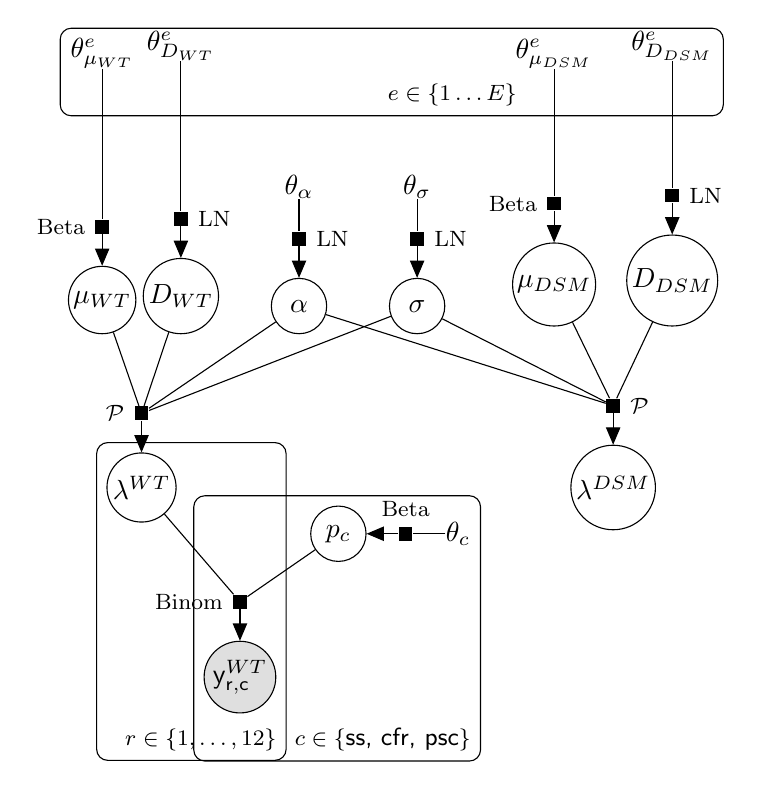
\begin{tikzpicture}[scale= 0.5]

  % Define nodes
  \node[obs]                               (y) {${\sf y}^{WT}_{\sf r,c}$};

 % PDE model output

	\node[latent, above=of y, yshift = 0.5cm, xshift = -1.25cm] (lambdaWT) {$\lambda^{WT}$};
	\node[latent, right=of lambdaWT,xshift = 4cm] (lambdaGE) {$\lambda^{DSM}$};

% Observation model parameters
	\node[latent, above=of y, yshift = 0.0cm, xshift = 1.25cm] (pC) {$p_{c}$};

% PDE model parameters

	\node[latent, above=of lambdaWT, xshift = -0.5cm, yshift = 0.5cm] (muWT) {$\mu_{WT}$};
	\node[latent, above=of lambdaWT, yshift = 0.5cm, xshift = 0.5cm] (deltaWT) {$D_{WT}$};

	\node[latent, above=of lambdaGE, yshift = 0.5cm, xshift = -0.75cm] (muGE) {$\mu_{DSM}$};
	\node[latent, above=of lambdaGE, yshift = 0.5cm, xshift = 0.75cm] (deltaGE) {$D_{DSM}$};

	\node[latent, above=of lambdaWT, yshift = 0.5cm, xshift = 2cm] (alpha) {$\alpha$};
	\node[latent, above=of lambdaWT, yshift = 0.5cm, xshift = 3.5cm] (sigma) {$\sigma$};
  
  
% Expert elicited parameters

  	\node[const, above=of muWT, yshift = 1.5cm] (thetaMu) {$\theta_{\mu_{WT}}^e$};
	\node[const, above=of deltaWT, yshift = 1.5cm] (thetaDelta) {$\theta_{D_{WT}}^e$};
	\node[const, above=of muGE, yshift = 1.2cm] (thetaMuG) {$\theta_{\mu_{DSM}}^e$};
	\node[const, above=of deltaGE, yshift = 1.2cm] (thetaDeltaG) {$\theta_{D_{DSM}}^e$};

% Other priors

	\node[const, right=of pC] (priorpC) {$\theta_{c}$};
	\node[const, above=of alpha] (priorAlpha) {$\theta_{\alpha}$};
	\node[const, above=of sigma] (priorSigma) {$\theta_{\sigma}$};

% Factors

\factor[above=of lambdaWT] {wWT} {left:$\mathcal{P}$} {muWT,deltaWT, alpha, sigma} {lambdaWT} ;
\factor[above=of lambdaGE] {wGE} {right:$\mathcal{P}$} {muGE,deltaGE, alpha, sigma} {lambdaGE} ;

\factor[above=of y] {wY} {left:Binom} {lambdaWT,pC} {y} ;
\factor[above=of muWT] {wmuWT} {left:Beta} {thetaMu} {muWT} ;
\factor[above=of muGE] {wmuGE} {left:Beta} {thetaMuG} {muGE} ;
\factor[above=of deltaWT] {wdeltaWT} {right:LN} {thetaDelta} {deltaWT} ;
\factor[above=of deltaGE] {wdeltaGE} {right:LN} {thetaDeltaG} {deltaGE} ;
\factor[right=of pC] {wthetapC} {above:Beta} {priorpC} {pC} ;
\factor[above=of alpha] {wthetaAlpha} {right:LN} {priorAlpha} {alpha} ;
\factor[above=of sigma] {wthetaSigma} {right:LN} {priorSigma} {sigma} ;

  % Plates
  \plate {expert} {(thetaMu.west)(thetaMu.north)(thetaDeltaG.east)(thetaMu.south)} {$e \in \{ 1\dots E\}\hspace{2.5cm}$};
  \plate {catchType} {(y)(pC)(priorpC)} {$c \in \{ \textsf{\small ss, cfr, psc}\}$};
  \plate {mrr} {(y)(lambdaWT)(catchType.west)} {$r \in \{1, \dots, 12\}$} ;

\end{tikzpicture}

\caption{\label{fig:bhm_schematic} Hierarchical structure of the model for the WT males observations and its connection to the DSM mosquitoes spread and persistence prediction. The parameters $\alpha$ (chemotaxis attraction strength) and $\sigma$ (chemotaxis attraction range) are shared between the two strains.}
\end{figure}

For a given release \emph{r}, we describe the number of available released mosquitoes at time $t$ as a Poisson random variable with expectation $\lambda_r(t)$, where the dependence of this expectation on location is suppressed:
\begin{eqnarray}
n_r(t) | \lambda_r(t) &\sim& \textrm{Poisson}(\lambda_r(t))
\end{eqnarray}
where $\lambda_r(t)$ is given by the PDE model described in Eq. \ref{mod3}. The data ${\sf y}$ are the observed count of male mosquitoes in a given trap. Since the traps catch only a portion of the mosquitoes that occur in their immediate vicinity, a natural trap observation model is the Binomial distribution:
  \begin{eqnarray}
{\sf y_{r,c}} | n_r, p_c &\sim& \textrm{Binomial}(n_r, p_c)
\end{eqnarray}
where $n_r$ is a realization of the Poisson random variable $\lambda_r$ (the expected number of released mosquitoes in the trap's immediate vicinity), and $p_c$ is the catchability parameter, or ``trap efficiency'', which is trap dependent. In this study we do not account for the possibility of false positive (insects or mosquito species incorrectly identified as released male mosquitoes) or false negative (released male \textit{An. gambiae} mosquitoes incorrectly identified as something else) probabilities as they are assumed to be equal to $0$ \citep{Epopa2017}.

Given the  binomial likelihood, the posterior distribution is obtained by integrating over the possible Poisson outcomes:
  \begin{eqnarray}
{\bm \pi}(\theta_d, \lambda_r, {p_c} | {\sf y}) &\propto & \prod_c \prod_r \Big[ \sum_{n_r}  \underbrace{{\bm \pi}({\sf y_{r,c}} | n_r, p_c) {\bm \pi}(n_r | \lambda_r)}_{data}  \Big] \underbrace{{\bm \pi}(\lambda_r | \theta_d)}_{process} \underbrace{{\bm \pi}( \theta_d)}_{prior} 
\end{eqnarray}

Markov Chain Monte Carlo (MCMC) inference methods have been successfully applied to hierarchical Bayesian models, similar to the model described here, on many occasions \cite[see for example][]{McGoff2012a, Chkrebtii2016, Wikle2003, Ruggeri2017}. We found, however, that the standard random-walk Metropolis MCMC routine was too slow to mix. Furthermore in this context, more advanced methods such as Hamiltonian Monte Carlo sampling, which require repeated likelihood computations along the proposal path, are inefficient because of the high computational costs entailed by the need to numerically solve the PDE model for each new proposal. 

We found a reasonable compromise through the delayed rejection adaptive Metropolis algorithm DRAM, proposed by \cite{Haario2001a}. This MCMC algorithm uses a multivariate proposal distribution that automatically adapts to allow for posterior correlations between the parameters and identifies the directions of principal change along the ridges in the posterior surface. The acceptance rate of the DRAM algorithm is also improved by using a delayed rejection scheme where, instead of immediately advancing the chain following rejection of a parameter set, a second proposal is made that depends on both the current position of the chain and the rejected parameter set. We implemented DRAM by using the function modMCMC in the FME package \cite{Soetaert2010} in R (R Core Team, 2015), using one delayed rejection step, and updating the proposal distribution every 200 iterations. We run a total of $3$ MCMC chains of $15000$ samples each, with $5000$ used as burn-in. The convergence of the chains was assessed using Gelman's $\hat{R}$ criterion \citep[see ][chapter 11]{Gelman2014}.

\subsection{Posterior prediction validation} 
We evaluated the accuracy of the posterior model predictions by comparing them against the observed recaptures in the MRR experiment that we deliberately withheld from the inference procedure. The fifth MRR experiment was conducted at the same location as the first four experiments, and under similar conditions with two exceptions: (i) all marked male mosquitoes were released at a single location; and, (ii) a much larger number of mosquitoes were released (Table~\ref{tab:relLoc}). The experimental conditions and population dynamics might therefore be considered to be slightly different than those that prevailed during the first four experiments. If the model is nonetheless able to make sufficiently accurate predictions, then we may be more confident in its ability to be generalized to other similar release scenarios.

\subsection{Bayesian model averaging}
The field data for the WT male mosquito allows us to calculate the posterior distribution for the WT mortality and dispersal distance parameters. This in turn allows us to measure how well each expert's prior distribution matches the posterior distribution, and weight each expert's response accordingly. We do this by considering each expert's prior as an alternative model, and use the theory of model evidence \cite{robert2001bayesian} to calculate the Bayes factor \citep{Kass1995b, Hosack2020}. 

We assume that experts who are good at predicting outcomes with WT mosquitoes (i.e. those whose prior distributions are close to the posterior distributions) will also be good at predicting outcomes with DSM mosquitoes, and weight the experts' DSM priors by the posterior probability of the models using Bayesian model averaging to obtain a weighted linear pool of expert opinion for the DSM mortality and dispersal distance.

\section{Results}
\subsection{WT parameters}
Table \ref{tble:sumStatPPpost} provides the summary statistics of the posterior distributions of the PDE model parameters (Figure \ref{fig:prior_posterior} provides both the priors and posteriors for comparison). The use of the MRR data allowed us to provide refined estimates for the parameters of the PDE model. The diffusion coefficient in particular has seen its uncertainty decrease, yielding a mean value of 127 m$^2$ per day. The chemotaxis component has a posterior mean value of about $0.07$, while the range parameter for the mosquito attraction is about $33.9$ m.\\

The posterior samples of the dispersal and swarm attraction parameters are highly correlated such that high dispersal values are associated with low attraction, and vice-versa. We anticipated this and deliberately chose a weakly informative prior for the attraction parameter to allow the data to drive their posterior estimates as far as possible. The largest observable dispersal, however, is clearly dictated by the distance between the sources of attractant (compounds) and the traps laid out in the field. In this instance, all traps were laid within 500m of release sites and compounds \citep[Figure 1]{Epopa2017} limiting the ability to infer the possibility of the much higher dispersal values represented in the expert prior (Figure~\ref{fig:prior_posterior}).

\begin{figure}[t]
%\centering{ \includegraphics[width=0.95\textwidth]{./figure/paramPriorsSpread-1.png}}
\centering{ 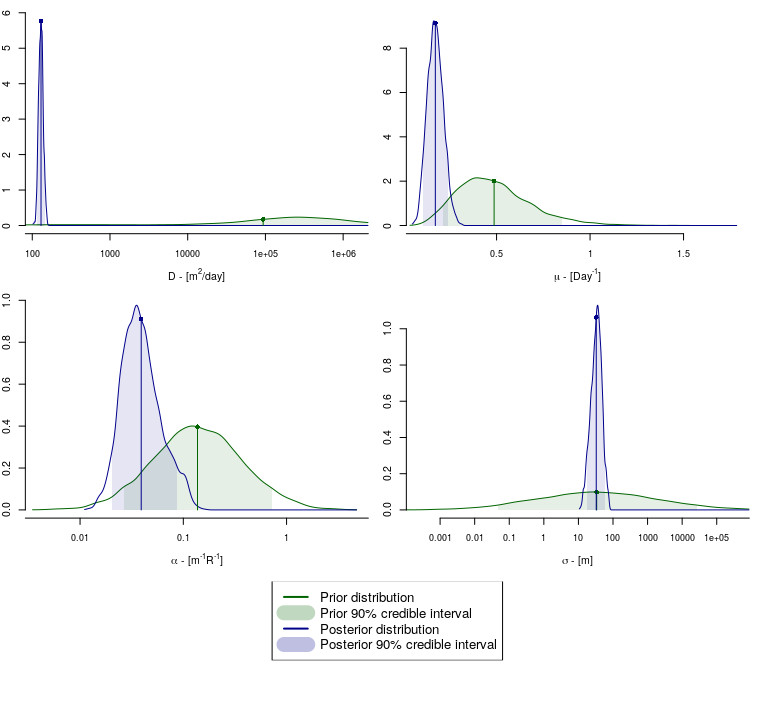
\includegraphics[width=0.95\textwidth]{./Figure2.png}}
\caption[Plot of the prior and posterior distributions for the four PDE model parameters.]{Plot of the prior and posterior distributions for the four PDE model parameters.}\label{fig:prior_posterior}
\end{figure}

\begin{table}[h]
\centering
\begingroup\small
\begin{tabular}{|c|ccc|}
\hline
Parameter & Mean & Q05 & Q95 \\\hline
Mortality - $\mu$ & 0.16 (0.14) & 0.11 (0.10) & 0.24 (0.21)\\
Diffusion - $D$ & 127.0 & 113.7 & 140.7\\
Swarm attraction - $\alpha$ & 0.07 & 0.03 & 0.10\\
Swarm range - $\sigma$ & 33.9 & 19.8 & 56.1\\
Catchability psc - $p_{psc}$ & 0.18 & 0.11 & 0.25\\
Catchability cfr - $p_{cfr}$ & 0.03 & 0.02 & 0.05\\
Catchability ss - $p_{ss}$ & 0.29 & 0.24 & 0.34\\
\hline
\end{tabular}
\endgroup
\caption{\label{tble:sumStatPPpost} Summary statistics for the posterior distributions of the PDE model parameters inferred from the WT MRRs. In brackets in the first line we added the equivalent daily mortality rate value, for ease of comparison with other studies.}
\end{table}

\subsection{Spread and persistence of male WT mosquitoes}
Figure \ref{fig:Post_Data} provides an overview of the expected evolution of the number of mosquitoes caught in the set of traps set for the fifth MRR. When comparing the model outcomes to the actual capture data, we note that of the 70 observations (number of mosquitoes caught in a given trap at a given time), only 2 are outside the $90\%$ credible interval given by the model, providing a good level of confidence on the ability of the model to capture the general dynamic, and its ability to make usable predictions both in space and time about the spread and dispersal of WT strain mosquitoes.  


\begin{figure}[t]
%\centering{ \includegraphics[width=0.95\textwidth]{./figure/Post_Data-1.png}}
\centering{ 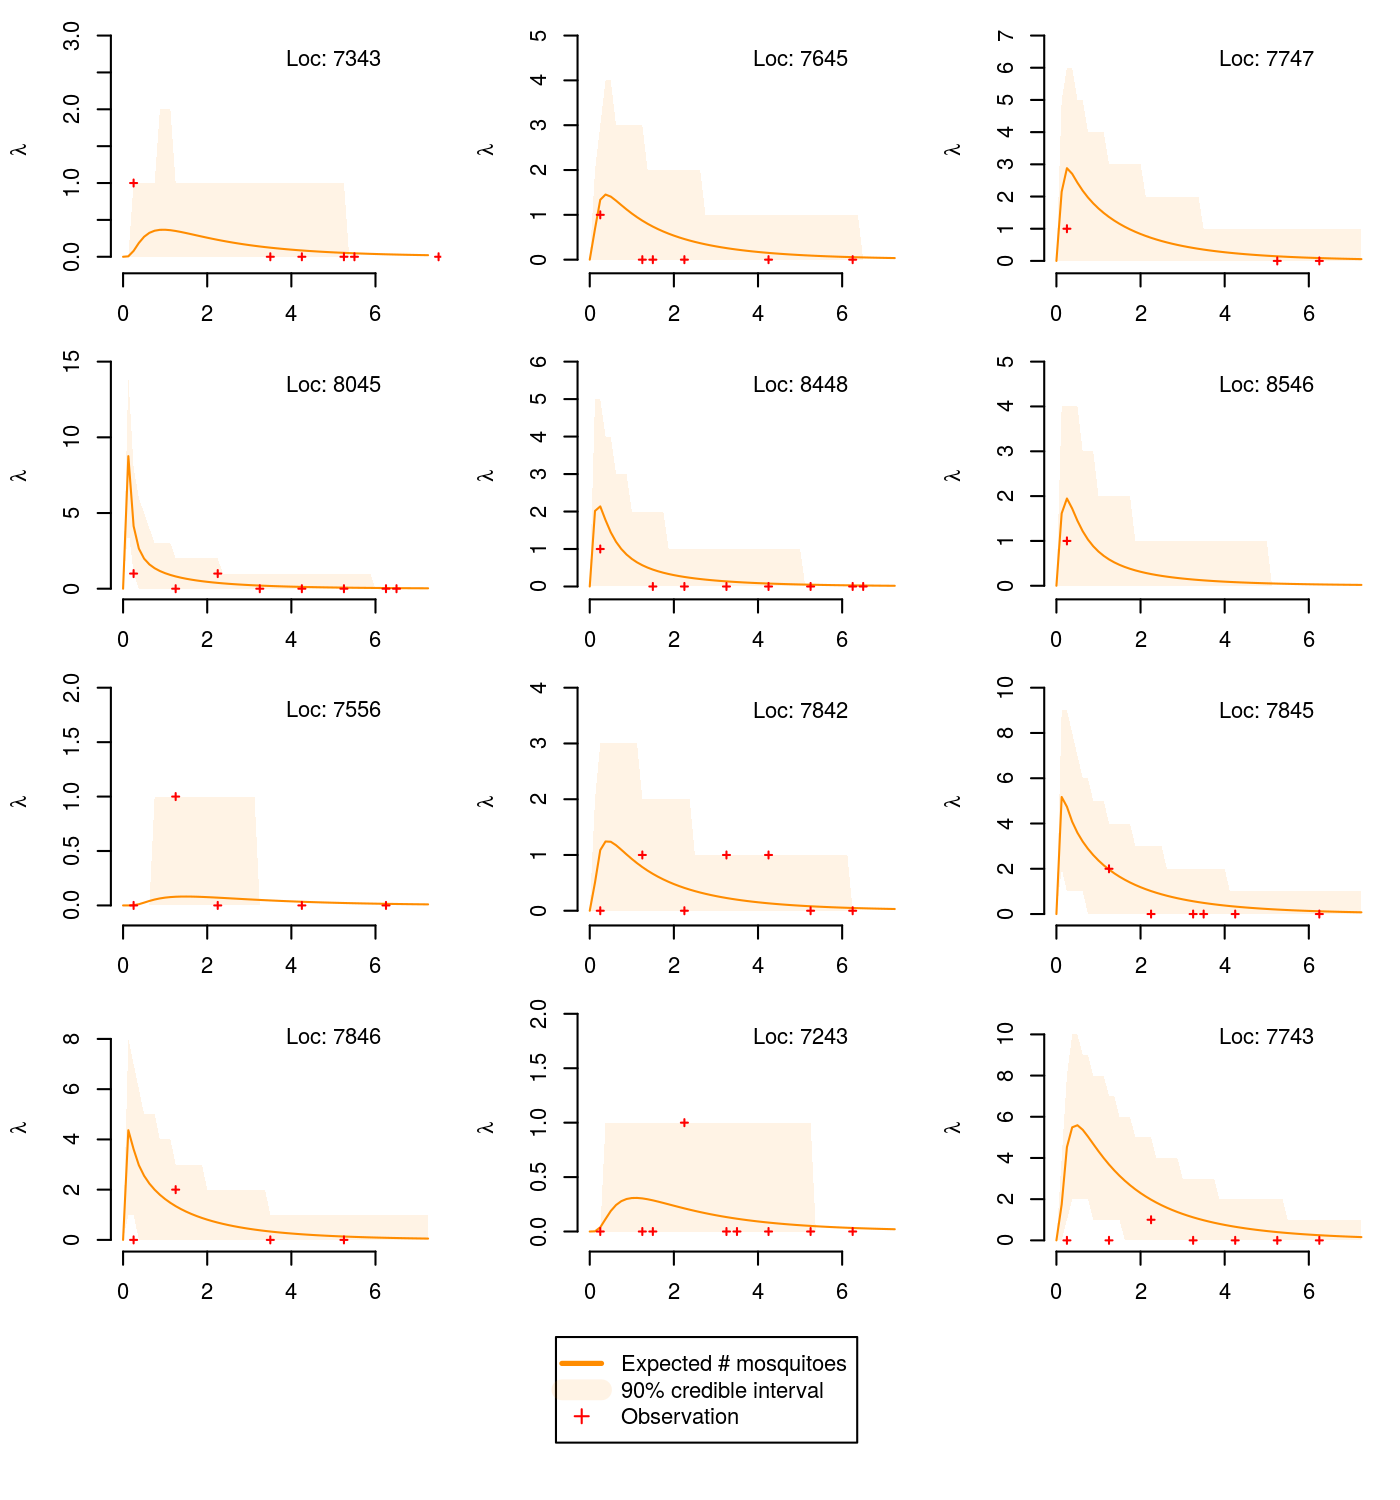
\includegraphics[width=0.95\textwidth]{./Figure3.png}}
\caption[Plot of the true observations (red crosses) and the expected number of catches (orange line) from the simulated model]{Plot of the true observations (red crosses) and the posterior predictive expected number of catches (orange line) from the simulated model, as a function of days. The orange shade represent the $90\%$ credible interval for the number of catches at the specified location. It is expected that $90\%$ of the red crosses falls within the orange polygon.}\label{fig:Post_Data}
\end{figure}

\subsection{DSM parameters}
The weighted linear pool priors for DSM mortality and diffusion (weighted according to the Bayesian model averaging approach detailed above) are summarised in Table \ref{tble:sumStatPPpostbma}. The two parameters are quite different from the WT posterior estimates, with the DSM mortality prior six times higher than the WT posterior, and the dispersal multiple orders of magnitude bigger. 

The difference between the posterior distributions for WT and DSM mortality reflects the effect of the Bayesian model averaging but also the significant reduction in uncertainty that occurs when moving from prior to posterior distributions (see Figure \ref{fig:prior_posterior}) as often occurs in a Bayesian analysis. The linear pool of expert prior distribution for the dispersal distance of WT mosquitoes was also very much higher than its posterior distribution estimated using the data. It is possible therefore that the weighted linear pool prior for DSM dispersal will also prove to be an overestimate, noting of course that the posterior estimates of WT dispersal are conditional on the design of the MRR experiments which was established before this analysis.

\begin{table}[h]
\centering
\begingroup\small
\begin{tabular}{|c|ccc|}
\hline
Parameter & Mean & Q05 & Q95  \\\hline
Mortality - $\mu$ & 1.05 (0.65) & 0.19 (0.17) & 2.42 (0.91)\\
Diffusion - $D$ & 753 $\times$ 10$^{3}$ & 8.77 & 112  $\times$ 10$^{4}$\\
\hline
\end{tabular}
\endgroup
\caption{\label{tble:sumStatPPpostbma} Updated statistics for the PDE model parameters using the WT MRRs results and the DSM priors. In brackets in the first line we added the equivalent daily mortality rate value, for ease of comparison with other studies.}
\end{table}

\subsection{Spread and persistence of male DSM mosquitoes}
The predicted persistence of DSM mosquitoes following a release of a single cohort of 5000 males is summarised in Figure \ref{fig:plotTimeMoxMaxLoc}. The large uncertainty captured in Table \ref{tble:sumStatPPpostbma} is clearly reflected in these predictions: the mean expected survival is estimated to be about 9 to 10 days, with a 90\% probability that the expected number of male DSM mosquitoes falls below 1 by Day 10. The 90\% credible interval, however, is large, and there is a small probability ($\sim 0.05$) that it could take as long about two months for this to occur.

\begin{figure}[t]
%\centering{ \includegraphics[width=0.95\textwidth]{figure/Persistence_SM.png}}
\centering{ 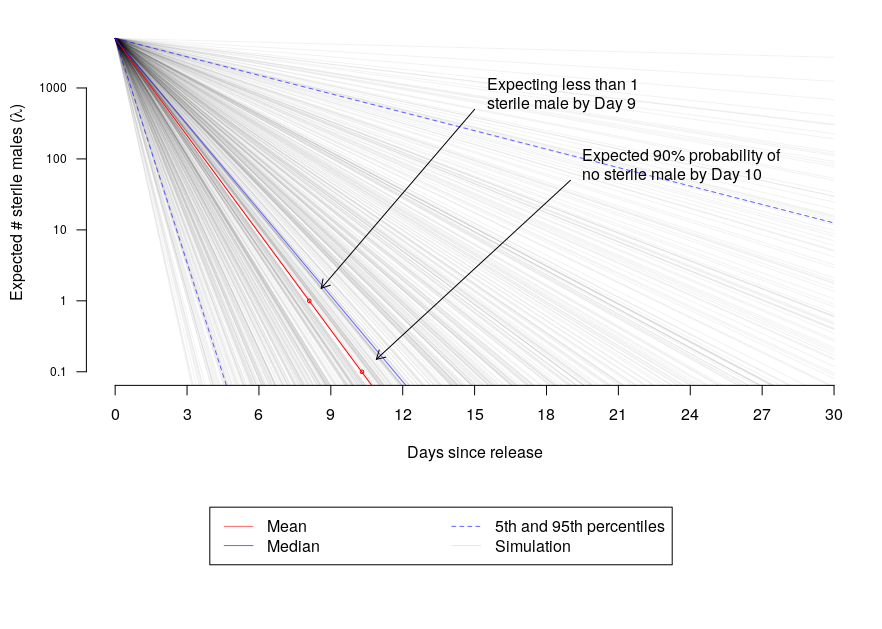
\includegraphics[width=0.95\textwidth]{./Figure4.png}}
\caption[Evolution of the expected number of mosquitoes following a release of $5000$ at location R]{ Evolution of the predictive posterior expected number of mosquitoes following a release of $5000$. Note that the scale of the y axis is logarithmic, making the model predictions linear.}\label{fig:plotTimeMoxMaxLoc}
\end{figure}

The dispersal of the DSM mosquitoes is balanced by the mortality rate. Because of this, the DSM are not expected to disperse far from their release site, with the expected number of mosquitoes per cell delineated by the red and orange contours in Figure \ref{fig:plotSpread}. For instance, while the spread is expected to extend on average to up to $500$m away from the release location by day $2$ (with at most a 1\% chance of finding a mosquito further away), the extent then contracts quickly to a limited area (less than $250$m from release location) by day $5$, to finally about $150$m away from the release location at day $12$.

\begin{figure}[t]
%\centering{ \includegraphics[width=0.95\textwidth]{figure/Spread_SM.png}}
\centering{ 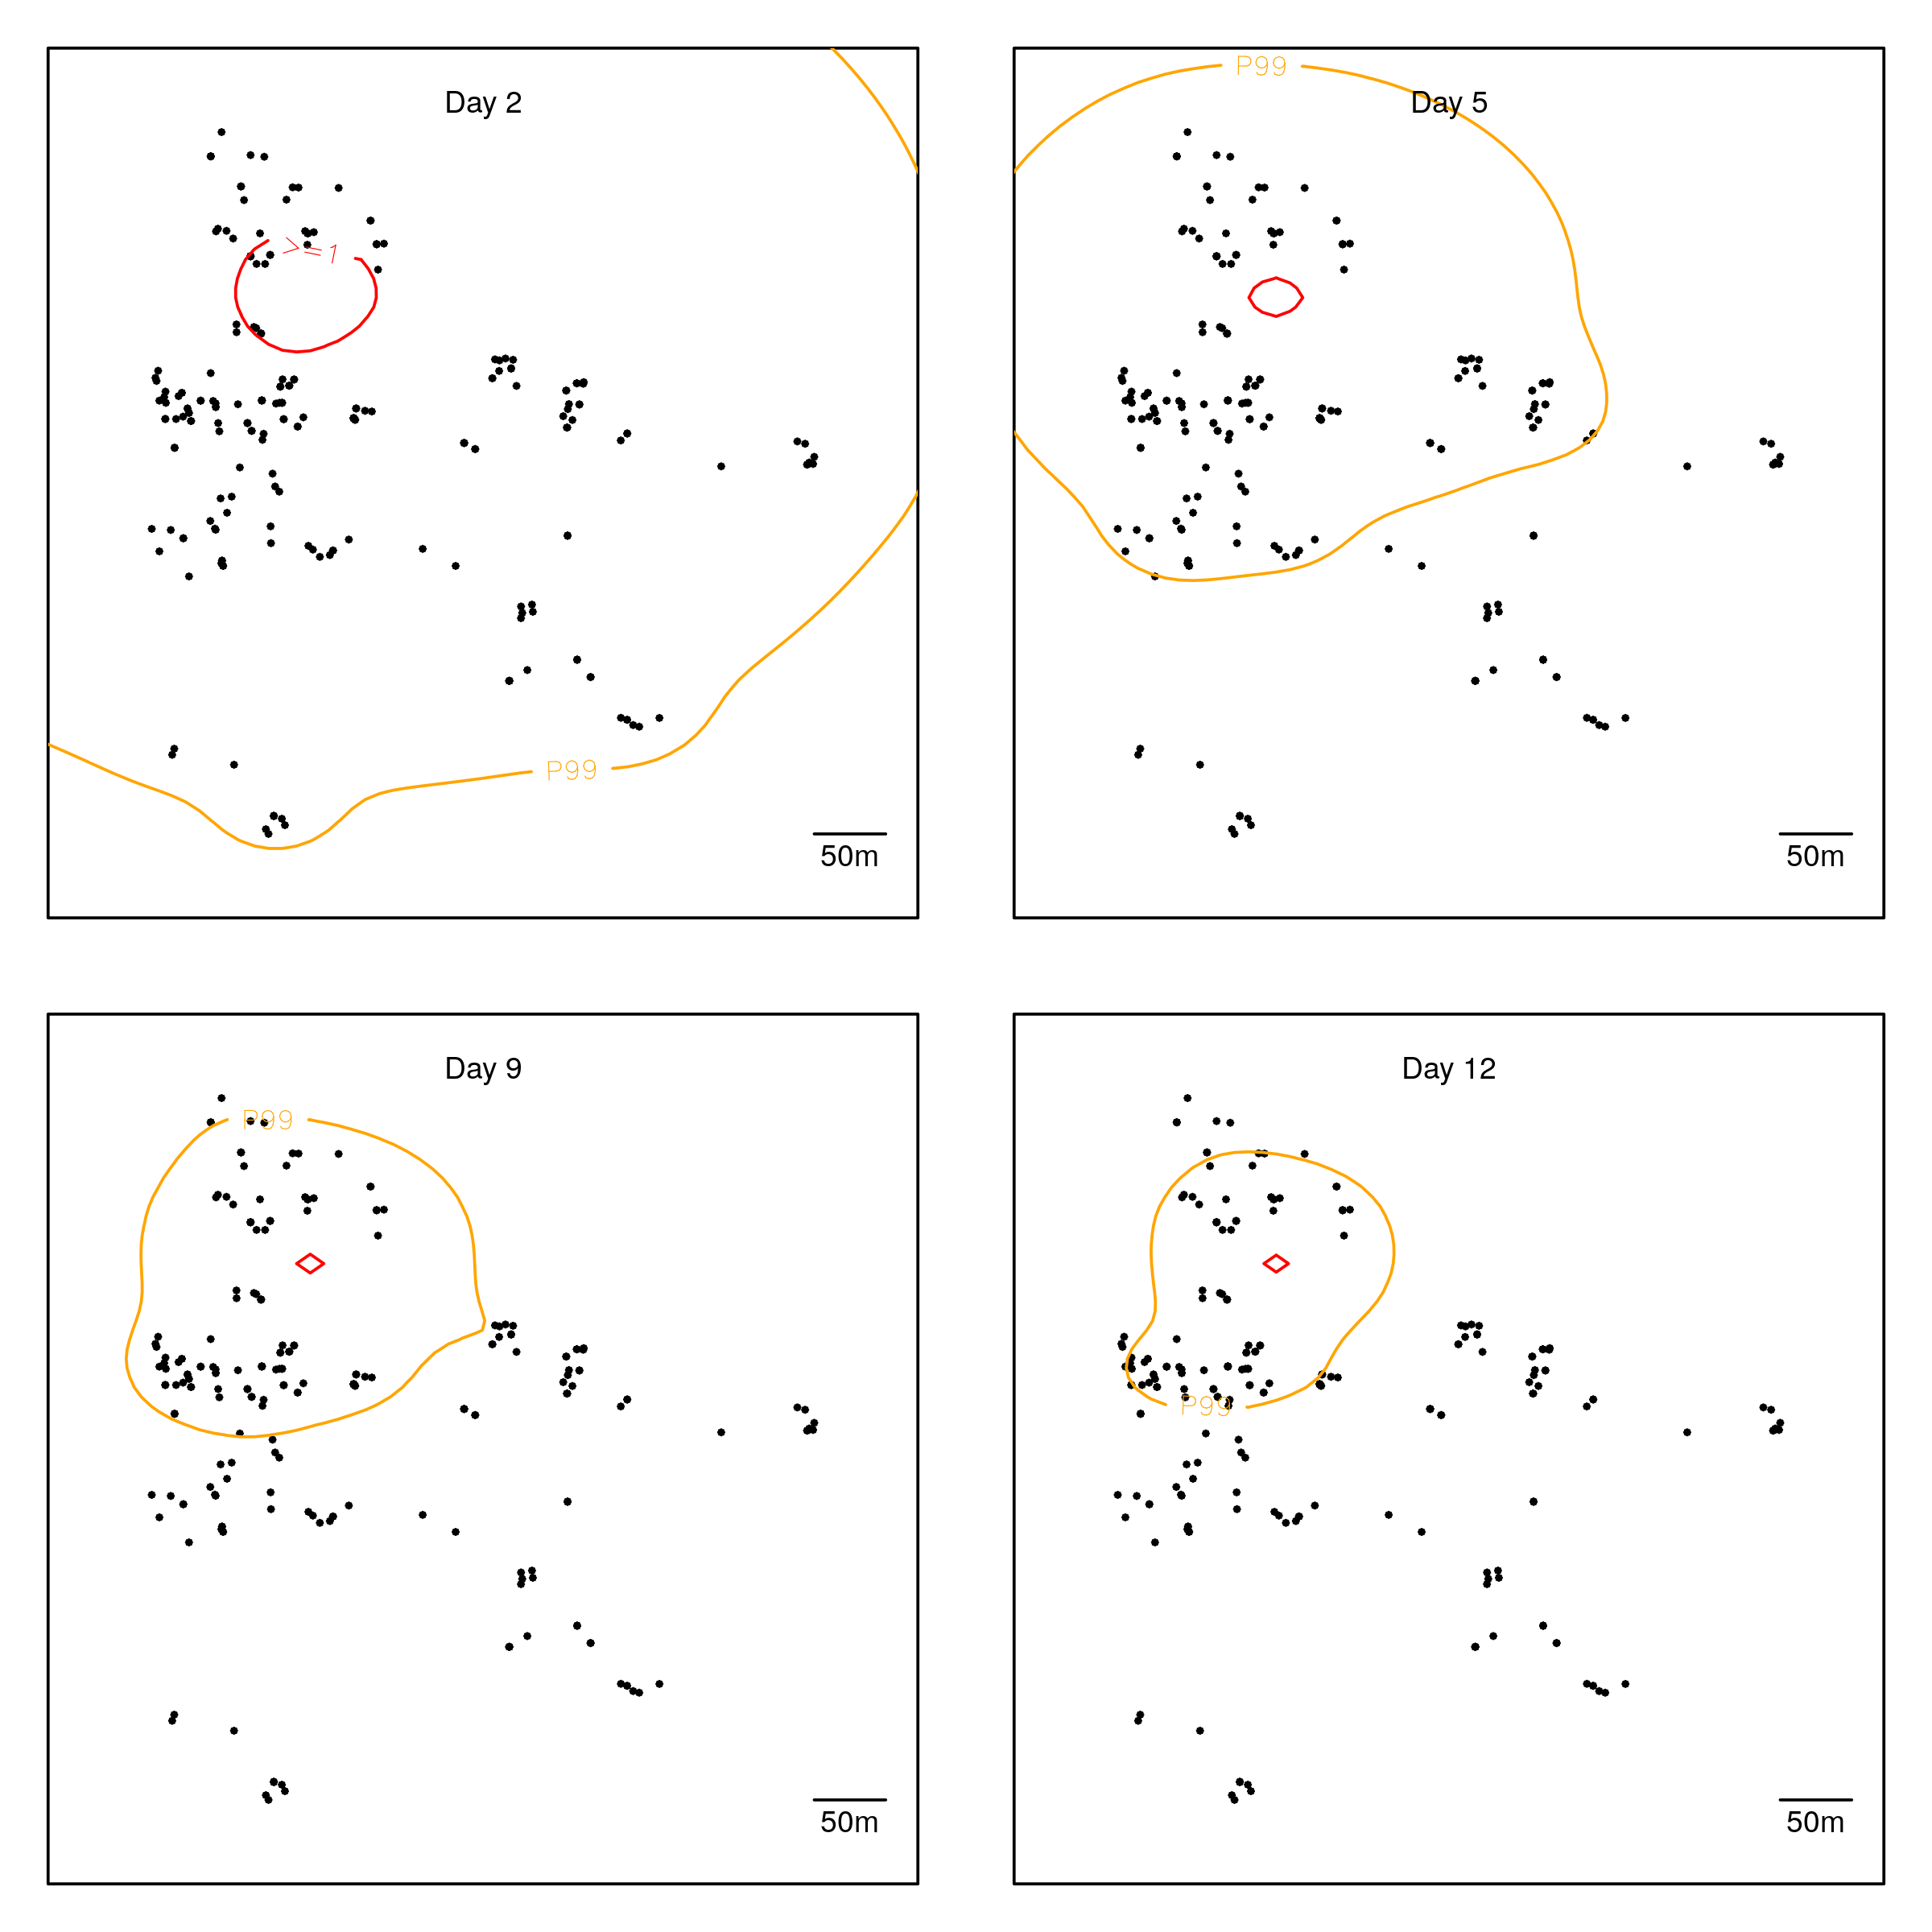
\includegraphics[width=0.9\textwidth]{./Figure5bis.png}}
\caption[Spread of the expected number of mosquitoes following a release of $5000$. Orange contour: outside the zone, the probablity of finding no DSM mosquito is $0.99$ or more. Red contour: inide the range, the expected number of DSM mosquito is $1$ or more.]{Spread of the predictive posterior expected number of mosquitoes following a release of $5000$. Orange contour: outside the zone, the probability of finding no DSM mosquito is $0.99$ or more. Red contour: inide the zone, the expected number of DSM mosquitoes is $1$ or more. Black dots: compounds locations.}\label{fig:plotSpread}
\end{figure}

\section{Discussion}
In this analysis we have used a combination of mathematical modeling, Bayesian inference, and expert elicitation to predict the spread and persistence of genetically modified DSM mosquitoes following the release of a single cohort of $5000$ individuals. These predictions were made as part of an independent risk assessment that was completed in May 2018 prior to the proposed field release \citep{Hayes2015a, Hayes2018}. The field release itself occurred in July 2019 (\href{https://tinyurl.com/y4qr9lc5}{See here}). We anticipate that the results from this field experiment will soon be forthcoming and provide an important opportunity to test the accuracy of the predictions presented here.

In this example we were able to validate the model predictions for wild type mosquitoes by holding back a proportion of the observation data. This also enabled us to use Bayesian model averaging to identify experts who were more accurate in their prior predictions. By allowing the opinions of these experts to carry greater weight we were also able to reduce uncertainty in the prior predictions for DSM mosquitoes. This approach assumes that experts who make more accurate predictions about wild type mosquitoes will also make better predictions about genetically modified mosquitoes. We will also be able to test this assumption once the results of the DSM field release are published.

Our results demonstrate how field observations greatly reduce the uncertainty between the prior information elicited with independent domain experts and the posterior distribution. Despite their relatively large uncertainty, however, our experience is that expert-derived prior distributions are essential when attempting to run inference over the multi-dimensional parameter space that dynamic population models demand, and that careful elicitation will therefore continue to be an essential component of future risk assessment studies.

Our posterior estimates of WT dispersal are conditional on a series of MRR experiments that were conducted prior to the elicitation of the dispersal prior distributions. These priors played no part in the experimental design, and the difference between the prior and posterior distributions depends on this design. This difference may reflect conservative prior estimates of mosquitoes' mean daily dispersal when in the vicinity of attractants (swarm locations) but it may also be an artefact of the MRR design that focussed efforts in and around village compounds to maximise the number of recaptures. As \cite{Epopa2017} notes, however, further intensive sampling studies outside or around villages will be useful to ensure that posterior estimates of dispersal are not blind to long range dispersal outcomes that are not witnessed because of the recapture site design.

We believe that dynamic population models will form a central component of any risk-based governance system for gene drive modified mosquitoes. We therefore suspect that confidence in this governance structure will likely depend on the extent to which risk assessments are able to predict the spread and persistence of mosquitoes carrying gene drive constructs, within the bounds of adequate accuracy. Critically, a staged release strategy provides the opportunity to compare the predictions of these types of models against observed outcomes, learn how to approach the modeling and inference challenges and gradually define the bounds of accuracy that are regulators and stakeholders believe are adequate.

This staged-learning is borne out by this analysis: the reproductive containment strategy utilised in the DSM mosquitoes provides a good, relatively simple, starting point for this type of analysis. The reaction dynamics in our model are greatly simplified by virtue of the fact that the released mosquitoes are sterile. The dynamic models for the second stage in Target Malaria's pathway, namely self-limiting male bias strains, will be more complicated because they must accommodate the birth processes and genetic dynamics that are not relevant here, and also other potentially important inter-specific interactions \citep{Beeton2020}. The models for the third and final stage, that is self-sustaining driving male bias strains, will be more complicated again particularly because the inter-specific interactions are likely to be more important and because the spatio-temporal scope of the analysis will be significantly larger.

Our analysis demonstrates the strength of the Bayesian approach in this context. Given its qualities, we believe this paradigm is the most appropriate to handle the prediction and risk assessment challenges that novel, gene drive-based strategies for controlling malaria vectors will pose in the coming years.

%%%%%%%%%%%%%%%%%%%%%%%%%%%%%%%%%%%%%%%%%%%%%%
%%                                          %%
%% Backmatter begins here                   %%
%%                                          %%
%%%%%%%%%%%%%%%%%%%%%%%%%%%%%%%%%%%%%%%%%%%%%%

\begin{backmatter}

\section*{Declaration}

\subsection*{Acknowledgements}
 This study would not be possible without the contribution of the domain experts - Heather Ferguson, Tovi Lehmann and Fred Gould; The authors would also like to acknowledge the numerous discussions and feedback received from Ron Thresher, Uffe Høgsbro Thygesen and Peter Caley. The authors would like to thank Jess Ford, Jeff Dambacher and Anders Gonçalves da Silva for helping facilitate the expert elicitation sessions. This analysis was funded by the Foundation for the National Institutes of Health and CSIRO Health and Biosecurity. The authors would also like to acknowledge CSIRO Data61 and Target Malaria for their help and support.


\subsection*{Author's contributions}
AI carried out the original draft preparation, proposed the statistical model and ran the statistical analyses; SF wrote the code for the PDE model. KH and GH participated in expert elicitation. All authors participated on drafting and revision of the manuscript. All authors gave final approval for publication and 
agree to be held accountable for the work performed herein.

\subsection*{Funding}
Not applicable.

\subsection*{Consent for publication}
Not applicable.

\subsection*{Competing interests}
The authors declare that they have no competing interests.

\subsection*{Ethics approval and consent to participate}
All elicitations were conducted with the informed consent of independent experts under ethics approval from the CSIRO Social Science Human Research Ethics Committee (reference LR06/2014). The mark release capture data was kindly provided by the Institut de Recherche en Sciences de la Sant\'{e}, Bobo-Dioulasso, Burkina Faso, and was collected with approval from the local institutional ethics committee (Centre Muraz Institutional Ethics Committee), reference number 009–2012/CE-CM.

\subsection*{Availability of data and material}

The datasets used and/or analysed during the current study are available from the corresponding author on reasonable request. The code used to generate the results is accessible from the following github repository \href{https://github.com/ick003/rRiskDSMspread}{rRiskDSMspread}.

%%%%%%%%%%%%%%%%%%%%%%%%%%%%%%%%%%%%%%%%%%%%%%%%%%%%%%%%%%%%%
%%                  The Bibliography                       %%
%%                                                         %%
%%  Bmc_mathpys.bst  will be used to                       %%
%%  create a .BBL file for submission.                     %%
%%  After submission of the .TEX file,                     %%
%%  you will be prompted to submit your .BBL file.         %%
%%                                                         %%
%%                                                         %%
%%  Note that the displayed Bibliography will not          %%
%%  necessarily be rendered by Latex exactly as specified  %%
%%  in the online Instructions for Authors.                %%
%%                                                         %%
%%%%%%%%%%%%%%%%%%%%%%%%%%%%%%%%%%%%%%%%%%%%%%%%%%%%%%%%%%%%%

% if your bibliography is in bibtex format, use those commands:
\bibliographystyle{vancouver} % Style BST file (bmc-mathphys, vancouver, spbasic).
\bibliography{Publications-Writing-SpreadMozzies}     % Bibliography file (usually '*.bib' )
% for author-year bibliography (bmc-mathphys or spbasic)
% a) write to bib file (bmc-mathphys only)
% @settings{label, options="nameyear"}
% b) uncomment next line
%\nocite{label}

% or include bibliography directly:
% \begin{thebibliography}
% \bibitem{b1}
% \end{thebibliography}

%%%%%%%%%%%%%%%%%%%%%%%%%%%%%%%%%%%
%%                               %%
%% Figures                       %%
%%                               %%
%% NB: this is for captions and  %%
%% Titles. All graphics must be  %%
%% submitted separately and NOT  %%
%% included in the Tex document  %%
%%                               %%
%%%%%%%%%%%%%%%%%%%%%%%%%%%%%%%%%%%

%%
%% Do not use \listoffigures as most will included as separate files

%\section*{Figures}
%  \begin{figure}[h!]
%  \caption{\csentence{Sample figure title.}
%      A short description of the figure content
%      should go here.}
%      \end{figure}
%
%\begin{figure}[h!]
%  \caption{\csentence{Sample figure title.}
%      Figure legend text.}
%      \end{figure}

%%%%%%%%%%%%%%%%%%%%%%%%%%%%%%%%%%%
%%                               %%
%% Tables                        %%
%%                               %%
%%%%%%%%%%%%%%%%%%%%%%%%%%%%%%%%%%%

%% Use of \listoftables is discouraged.
%%
%\section*{Tables}

%%%%%%%%%%%%%%%%%%%%%%%%%%%%%%%%%%%
%%                               %%
%% Additional Files              %%
%%                               %%
%%%%%%%%%%%%%%%%%%%%%%%%%%%%%%%%%%%
\newpage
\section*{Additional Files}

\subsection{Additional file 1 -- Elicitation process, questions and answers}

\paragraph{Elicitation of the mortality parameter}
The experts were interviewed in person and individually. They were asked the following question \emph{"What is the mortality rate of WT/DSM males mosquitoes once outside the insectary?"}, where the mortality rate could be elicited in terms of probability of  survival or death. Experts were able to also choose which quantiles of the PRIOR  parameter distribution they wanted to elicit. Table \ref{tble:elicit_mort} summarises the details of each expert's opinion. The experts answered either in terms of probability of survival ($p_S$) or  death ($p_d$), which then we transformed into the mortality parameter $\mu$ of the PDE model using the relationship $\mu = - \log( 1-p_D)$, or in case of survival $\mu = -\log p_S$.
\begin{table}[h]
\centering
%\begingroup\small
\begin{tabular}{|c|cccc|}
\hline
Mosquito & Parameter & Distribution & Quantiles & Values  \\\hline
Wild type & Mortality & beta & \{0.1, 0.9\} & \{0.1, 0.2\}\\
Wild type & Mortality & beta & \{0.05, 0.95\} & \{0.055, 0.165\}\\
Wild type & Survival & beta & \{0.15, 0.85\} & \{0.5, 0.75\}\\
Sterile male & Mortality & beta & \{0.05, 0.95\} & \{0.066, 0.198\}\\
Sterile male & Mortality & beta & \{0.05, 0.95\} & \{0.2, 0.9\}\\
Sterile male & Survival & beta & \{0.15, 0.85\} & \{0.3, 0.6\}\\
\hline
\end{tabular}
%\endgroup
\caption{\label{tble:elicit_mort} Elicited values for the probability of death / survival. }
\end{table}


\paragraph{Elicitation of the dispersion parameter}
The experts  were asked the following question \emph{"What is the average daily dispersal distance of a WT/DSM male mosquito?"}, where the dispersal distance was understood as the distance from the origin a mosquito could be found after a duration of 1 day. Experts were able to choose which quantiles of the prior parameter distribution they wanted to elicit. Table \ref{tble:elicit_disp} summarises the details of each expert's opinion. The relationship between the elicited parameter $d$ and the diffusion coefficient $D$ is given below.
\begin{table}[h]
\centering
%\begingroup\small
\begin{tabular}{|c|ccc|}
\hline
Mosquito & Distribution & Quantiles & Values  \\\hline
Wild type & lognormal & \{0.05, 0.95\} & \{0.01, 2.9\}\\
Wild type & lognormal & \{0.25, 0.75\} & \{0.02, 0.2\}\\
Sterile male & lognormal & \{0.05, 0.95\} & \{0.008, 2.32\}\\
Sterile male & lognormal & \{0.25, 0.75\} & \{0.01, 0.1\}\\
\hline
\end{tabular}
%\endgroup
\caption{\label{tble:elicit_disp} Elicited values for the average daily dispersal. }
\end{table}


\subsection{Additional file 2 -- Derivation of the relationship between the diffusion coefficient and the average dispersal distance}
Let $d$ be the average dispersal distance after $t$ days. In order to determine what prior on $D$ the prior elicited from $d$ gives us, we need to establish the relationship between these two variables. Given the elicitation question, we have 
$$ d = \int_{\mathbf{R}_{+}}  \sqrt{\langle x, x  \rangle} \times p(x) dx$$
where $p(x)$ is the probability to find the mosquito at location $x$, and $\langle x, x  \rangle$ is the Euclidean norm. This can be empirically estimated by 
$$ d = \frac{1}{n}\sum^n  \sqrt{\langle x_i, x_i  \rangle}$$
where $x_i$ is the location of a mosquito $i$ after $t$ days , given it has been release from $(0,0)$. If we note  $f(x)$ the daily dispersal distance :
$$ f(x) = \sqrt{\langle x, x  \rangle} $$
we can then express the above equation in terms of expectation (in the random variable sense): 
$$d = \mathsf{E}[ f(x)]$$ 
 Because we assume that the mosquito behaviour is governed by the PDE model described in the model section of the article, we can write:
$$p(X_t = x) = \frac{1}{4 \pi D t} \exp\Big\{-\frac{\langle x, x  \rangle}{4 D t}\Big\}$$
where $X_t$ is the random variable describing the location of that same released mosquito at time $t$, and $x$ is a given location in $\mathbb{R}^2$. 
So we have:
$$ \mathsf{E} \Big[ f(x) \Big] = \int_{\mathbb{R}^2} \frac{\sqrt{\langle x, x  \rangle}}{4 \pi D t} \exp\Big\{-\frac{\langle x, x  \rangle}{4 D t}\Big\} dx $$
We can perform a change of variable, $x_1 = r \cos(\theta)$ and $x_2 = r \sin(\theta)$ where $r \in [0, +\infty)$ and $\theta \in [0, 2 \pi]$:
$$ d = \int_{\mathbb{R_+}} \int_{[0, 2 \pi]} \frac{r^2}{4 \pi D t} \exp\Big\{-\frac{r^2}{4 D t}\Big\} dr d\theta $$ 
which yields:
$$ d = \int_{\mathbb{R_+}} \frac{r^2}{2 D t} \exp\Big\{-\frac{r^2}{4 D t}\Big\} dr $$
If we write $s^2 = 2 D t$, we recognize the expectation of a Rayleigh distribution, $\mathsf{E}[r] = s \sqrt{\frac{\pi}{2}}$, and so we have:
$$ d = \sqrt{D t \pi } $$ or equivalently
$$D = \frac{d^2}{\pi t}$$
\emph{Note: it is often found in the literature that the diffusion coefficient can also be expressed in terms of mean squared dispersal distance $d_2$. It can be approximated by $d_2 = \frac{1}{n}\sum^n  \langle x_i, x_i  \rangle$  - note that $d_2 \neq d^2$ - and using the same development we have $D = d_2/4 t$.}
\end{backmatter}
\end{document}
